\section{Numerical Experiments}\label{sec:exp} 
In what follows, \Cref{sec:exp1} is themed around the key insight obtained from \Cref{th:main}, i.e., the correlation of the gates lies at the heart of `what is learnt in a DNN with ReLUs'. In particular, we show that operations (such as permuting the layers, tiling cum rotation of the gates, and giving a constant `all-ones' input to the value network) that destroy the layer by layer computational structure do not degrade test performance. These operations lead to combinatorially many models and in all of them the test performance remains the same. In \Cref{sec:exp2} we throw light on the open question in [\citenum{randlabel}] on why test performance degrades due to upstream training with random labels. 
\subsection{Robustness of Gates: Destroying layer-by-layer structure does not affect performance}\label{sec:exp1}
In this experiment we show that information in the gates is invariant even if we destroy the layer-by-layer structure. We consider the three kinds of gates (or gating regimes) described below.\\
%\indent \quad$1.$ \textbf{Fixed Learnt:} We \emph{pre-train} the feature network (which is a DNN with ReLUs), then \emph{freeze} the weights of the feature network, and then train the value network. This way we can measure information in the gates of a trained DNN.\\
%\indent \quad$2.$ \textbf{Fixed Random:} We initialise the feature network at random, and then \emph{freeze} its weights and then train the value network. This way we can measure information in the gates of a DNN at initialisation. Here, the feature and value network can be either initialised with the same weights i.e., dependent initialisation (DI) or statistically independent weights  i.e., independent initialisation (II).\\
%\indent \quad$3.$ \textbf{Decoupled Learning:} We initialise the weights of the value and feature network statistically independent and then train both of them. For the gradient to flow through the feature network we use \emph{soft-gating}, i.e., $G(q)=\frac{1}{1+\exp({-\beta\cdot q})}$, with $\beta=10$. 

We make use of the deep gated network (DGN) setup shown in \Cref{fig:dgn-prior-new} (right) which is an improvisation of the DGN in prior work [\citenum{npk}] shown in \Cref{fig:dgn-prior-new} (left). In the current setup, {\bf{$G_{i_1},\ldots,G_{i_4}$ is a permutation of the $G_1,\ldots,G_4$}}, which gives $24$ models. Note that these \textbf{permutations destroy the layer by layer structure}. In the prior setup both value and feature networks have the same input $x\in\R^{\din}$. In the current setup, we have two separate inputs, $x^{\text{f}}\in\R^{\din}$ for the feature network and $x^{\text{v}}\in\R^{\din}$ for the value network. We set $x^{\text{f}}=x$ always, however, for $x^{\text{v}}$ there are \textbf{two modes} namely (i) \textbf{standard}: we set $x^{\text{v}}=x$ ,(ii) \textbf{`all-ones'}: we set $x^{\text{v}}=\mathbf{1}\in\R^{\din}$ (a tensor of all $1$'s). While the setup on the left is only one model, the setup on the right has $\mathbf{48=24\times 2}$ \textbf{different models}, where $24=\texttt{factorial}(4)$ is due to the gate permutations and $2$ is due the settings of $x^{\text{v}}$.
\begin{figure}[t]
\centering
\begin{minipage}{0.4\columnwidth}
\centering
\resizebox{\columnwidth}{!}{
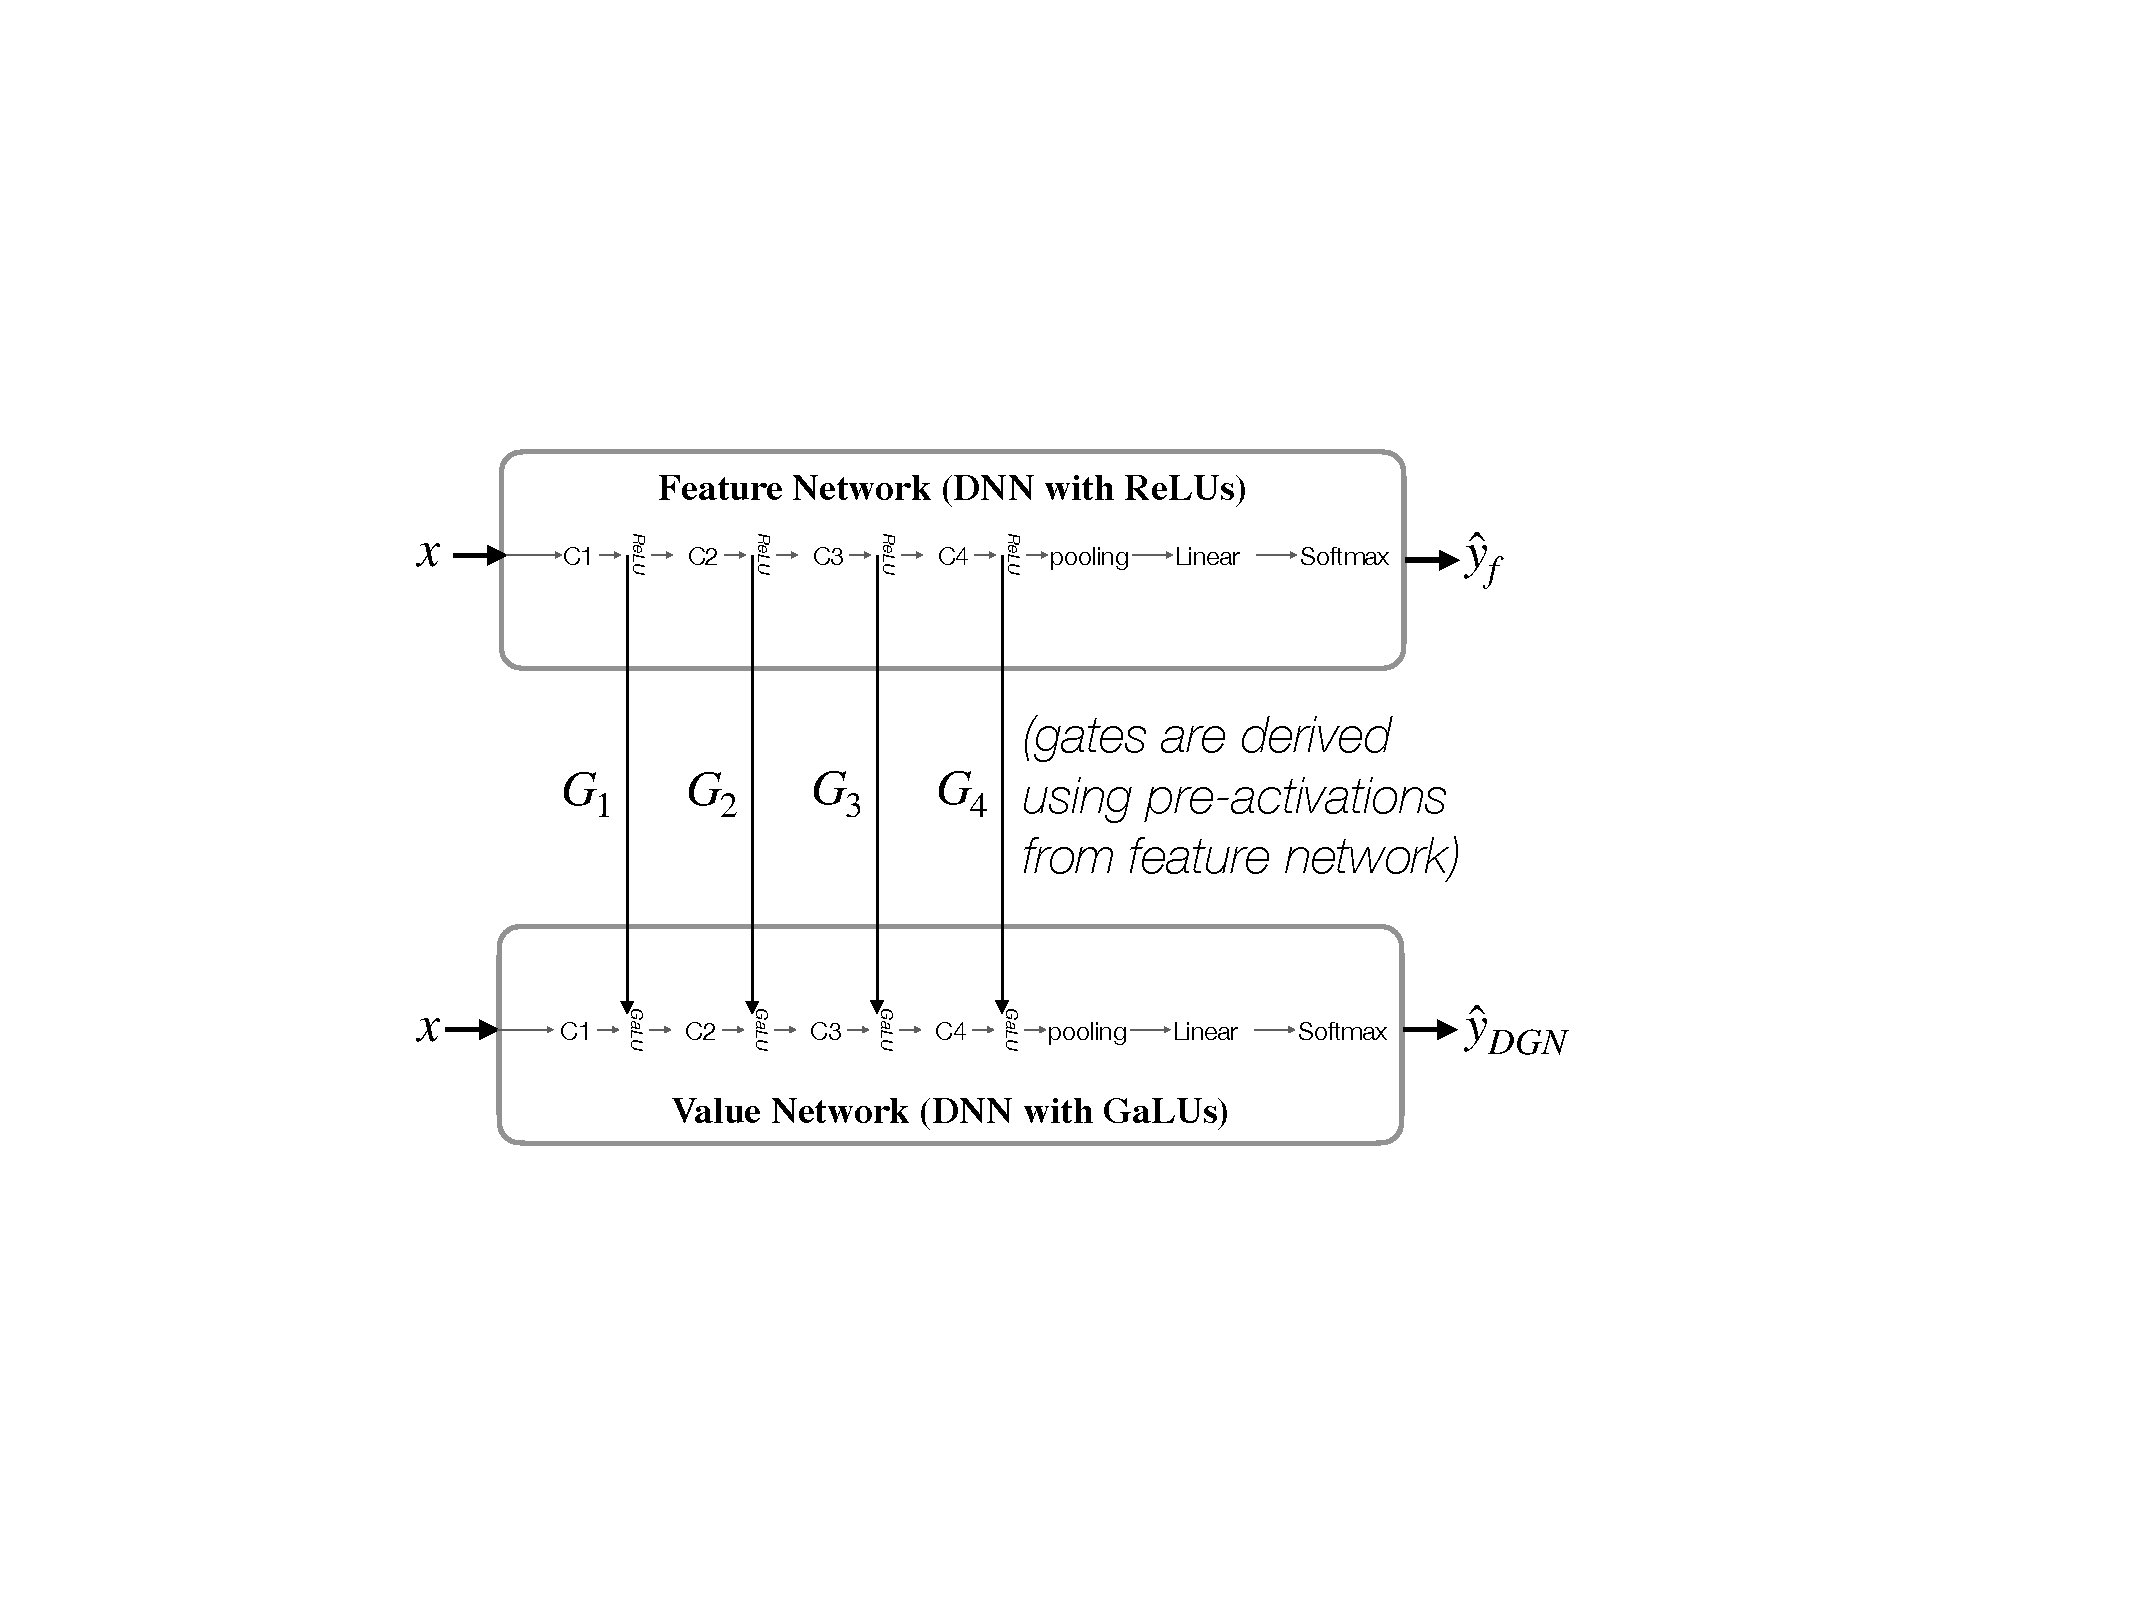
\includegraphics[scale=0.3]{figs/exp-prior.pdf}
}
\end{minipage}
\begin{minipage}{0.4\columnwidth}
\centering
\resizebox{\columnwidth}{!}{
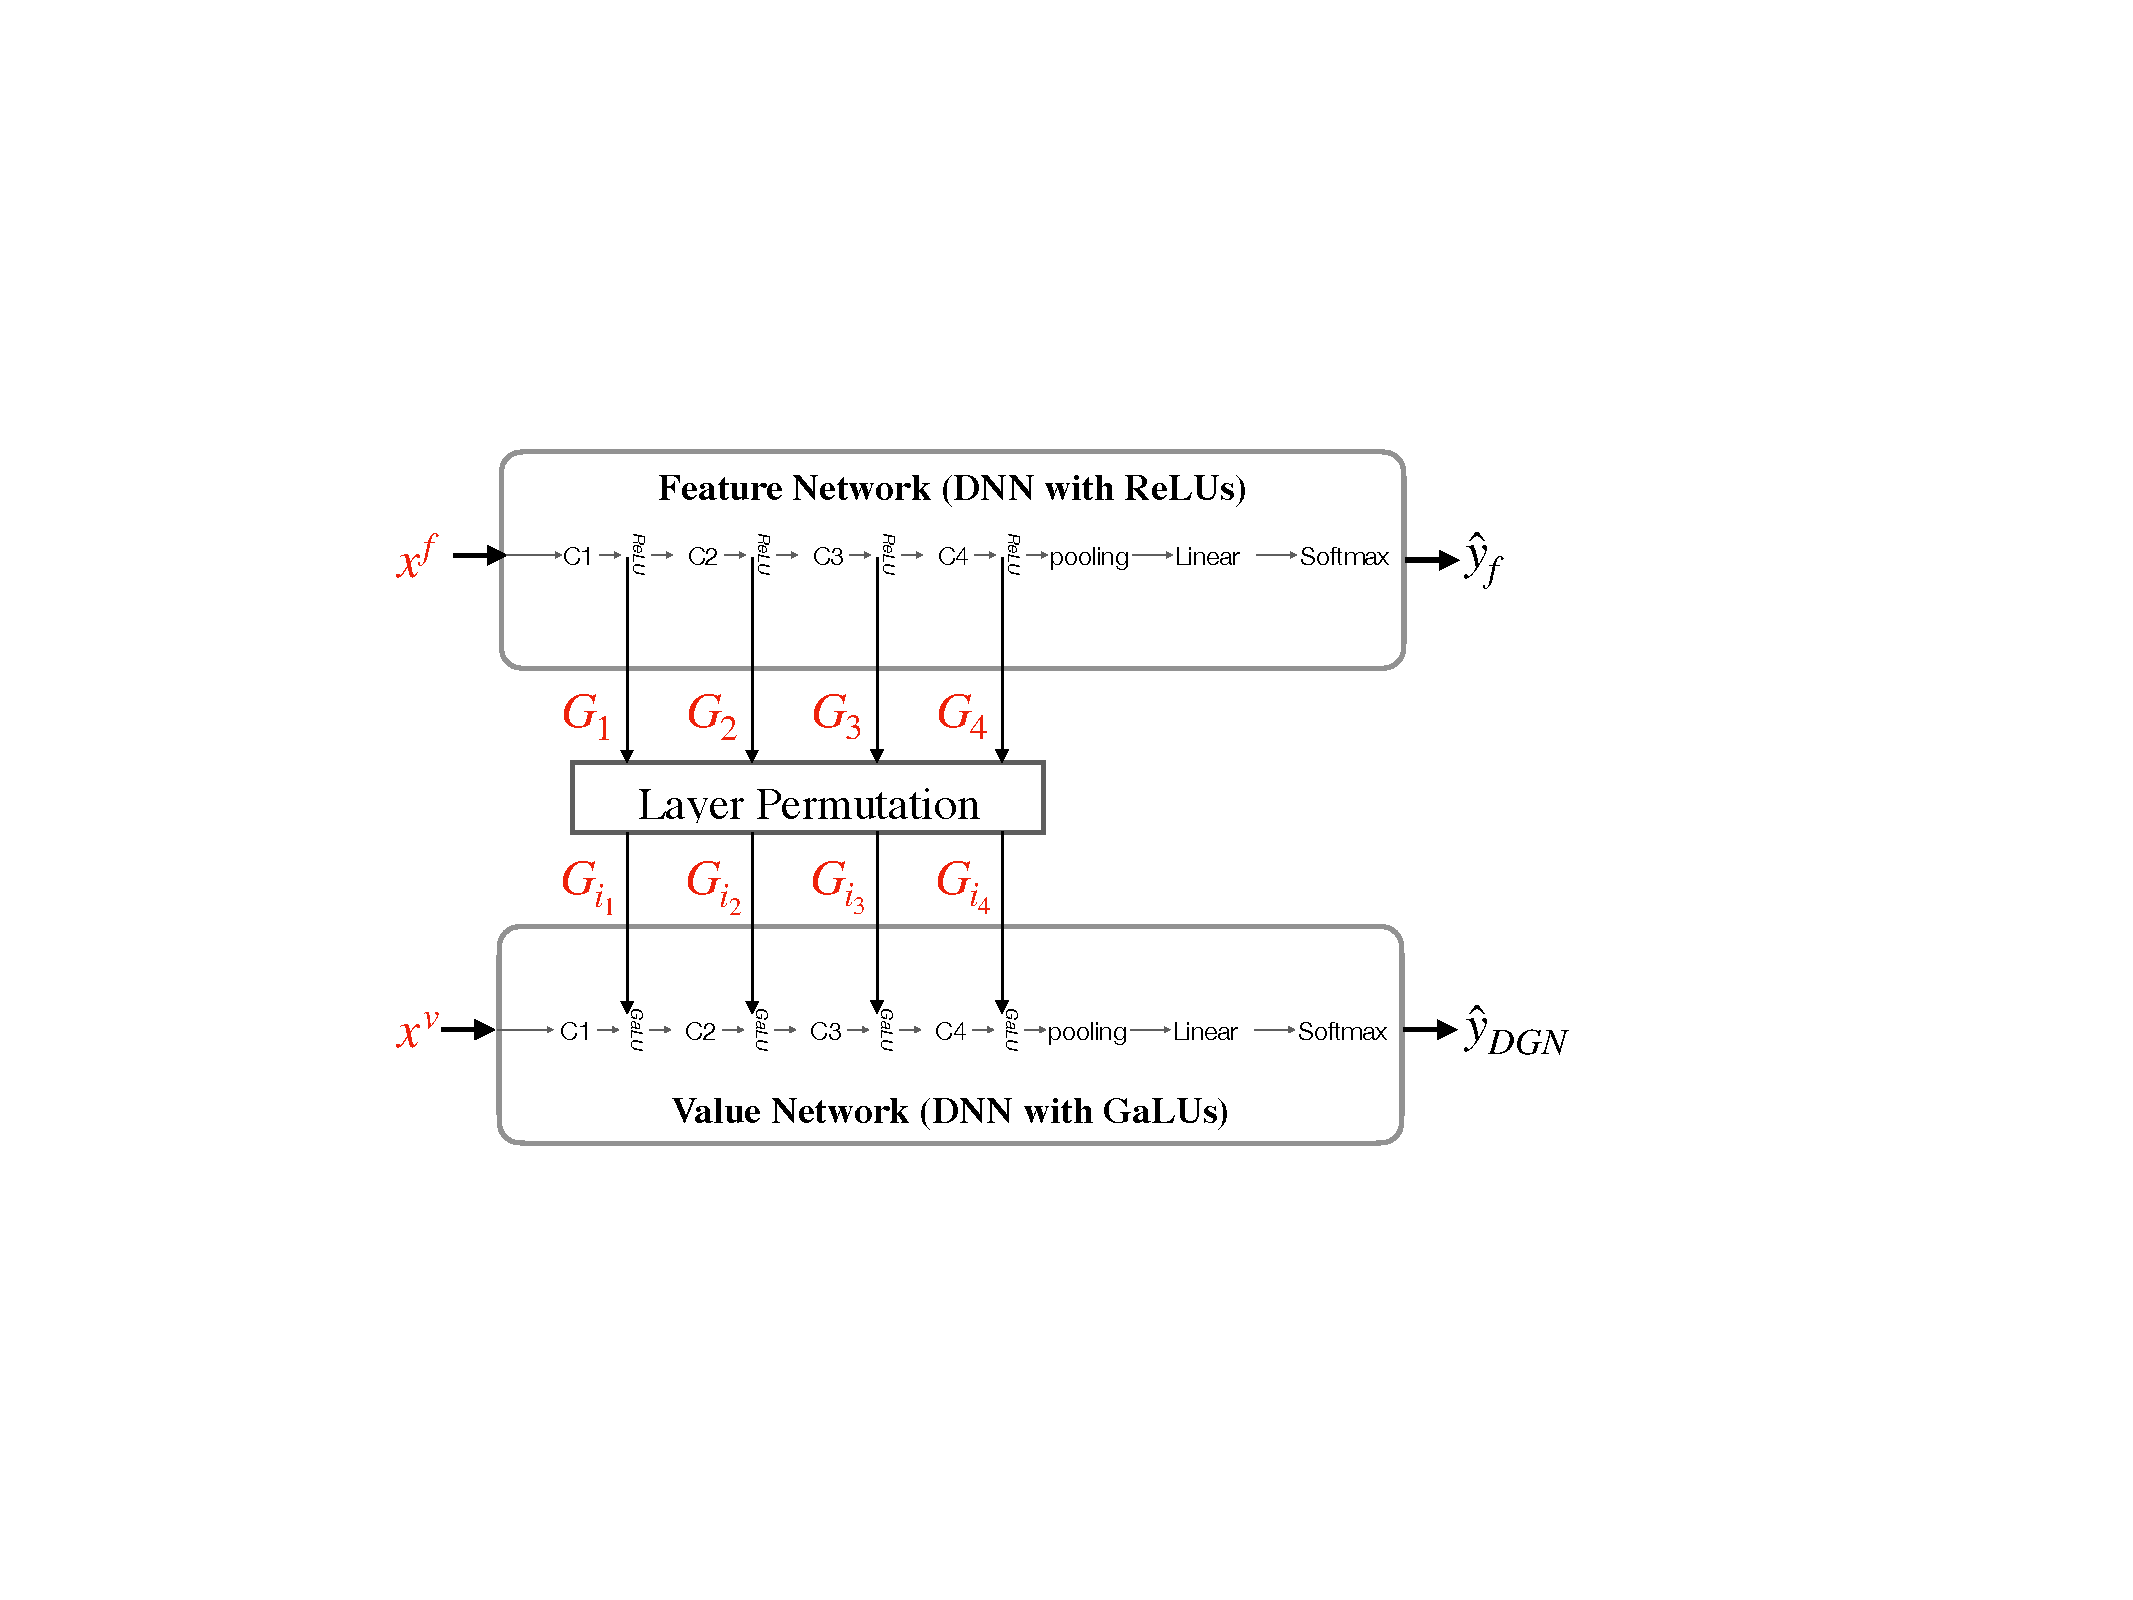
\includegraphics[scale=0.3]{figs/exp-new.pdf}
}
\end{minipage}
\caption{\small The prior setup in [\citenum{npk}] is shown in the left and the setup in this paper is shown in the right. Here $C1,\ldots,C4$ are convolutional layers with $128$ output filters, kernel size $3\times 3$ and stride $1\times 1$.}
\label{fig:dgn-prior-new}
\end{figure}
\begin{table}[t]
\centering
\begin{minipage}{0.95\columnwidth}
\begin{tabularx}{\columnwidth}{c *{5}{Y}}
\toprule
 Dataset& \multicolumn{2}{c}{Fixed Random}   &  \multicolumn{1}{c}{Decoupled} & \multicolumn{1}{c}{ Fixed } & \multicolumn{1}{c}{ReLU \tiny{(Feature Network)}}\\
& II & DI &Learning &Learnt &\\\hline\arrayrulecolor{white}\midrule
MNIST[\citenum{mnist}]& 94.1{\tiny{$\pm$0.3}}  &94.1\tiny{$\pm$0.3}  &98.1\tiny{$\pm$0.1} &98.6\tiny{$\pm$0.1} &98.5{\tiny{$\pm$0.1}}\\\hline\\\hline 
CIFAR-10[\citenum{cifar}]& 67.5\tiny{$\pm$0.7} &67.6\tiny{$\pm$0.7}   &77.6\tiny{$\pm$0.6} &79.4\tiny{$\pm$0.3} &80.4\tiny{$\pm$0.3}\\\hline
\arrayrulecolor{black}\bottomrule
\end{tabularx}
\end{minipage}
\caption{\small Shows the $\%$ test accuracy of various gates. The main result here is that the numbers in columns $1$ to $4$ are averaged over $48$ models (1 run per model, best performance in each run) and performance is robust to layer permutations and $x^{\text{v}}=\mathbf{1}$ input. For ReLU the average is over $5$ independent runs. Optimiser: Adam (3e-4). }
\label{tb:regimes}
\end{table}

\textbf{Note on prior results.} The following two observations were made in prior work [\citenum{npk}]: (i) by using the gates and training the NPV from scratch we can recover the performance (see ReLU vs Fixed Learnt in \Cref{tb:regimes}), and (ii) the performance of  Convolutional NTK ($77.43\%$)[\citenum{arora2019exact}] is between that of finite width network with random gates  ($67.5\%$) and learnt gates give ($79.4\%$), i.e., learning in the gates explains the difference between finite width DNNs and infinite width NTK.

\textbf{For `all-ones'} input to value network, in \Cref{th:main}, only $\ip{x,x'}=\din$, and $\Pi_{l=1}^{d-1}\frac{\ip{G_l(x),G_l(x')}}w$ is still unchanged. Similar explanations holds for \Cref{th:mainconv,th:mainres}.

\textbf{Robustness of Gates.} Entries in columns $1$ to $4$ in \Cref{tb:regimes} are  averaged over $48$ different models which included  permuting the layers and providing $\mathbf{1}$ as input. Our main result is that the information in the gates is robust over these $48$ models -- these justify the insights from \Cref{th:main} that as long as correlation in the gates is not destroyed the performance does not degrade. We also went one step further with respect to destroying the structure by considering arbitrary rotations. Here, we first tile the gates of the various filters (as a tensor) in the reverse order starting from layer $4$ to layer $1$ and then rotate arbitrarily in each of the three dimension for five times as shown in left of \Cref{fig:visual-permute} (i.e, two image dimensions and one filter dimension). For each rotation in the filter dimension we choose a random integer belonging to  $[0,512)$ and for each of the rotation in the image dimensions we choose a uniform random integer belonging to $[0,32)$. We did $10$ independent runs of the `fixed learnt' gates and `decoupled learning' of gates and observed the test performance to be $79.4${\tiny$\pm$0.2} and $79.0${\tiny$\pm$0.5} respectively (which are similar to the numbers shown in \Cref{tb:regimes}).

\begin{figure}[t]
\begin{minipage}{0.25\columnwidth}
\resizebox{\columnwidth}{!}{
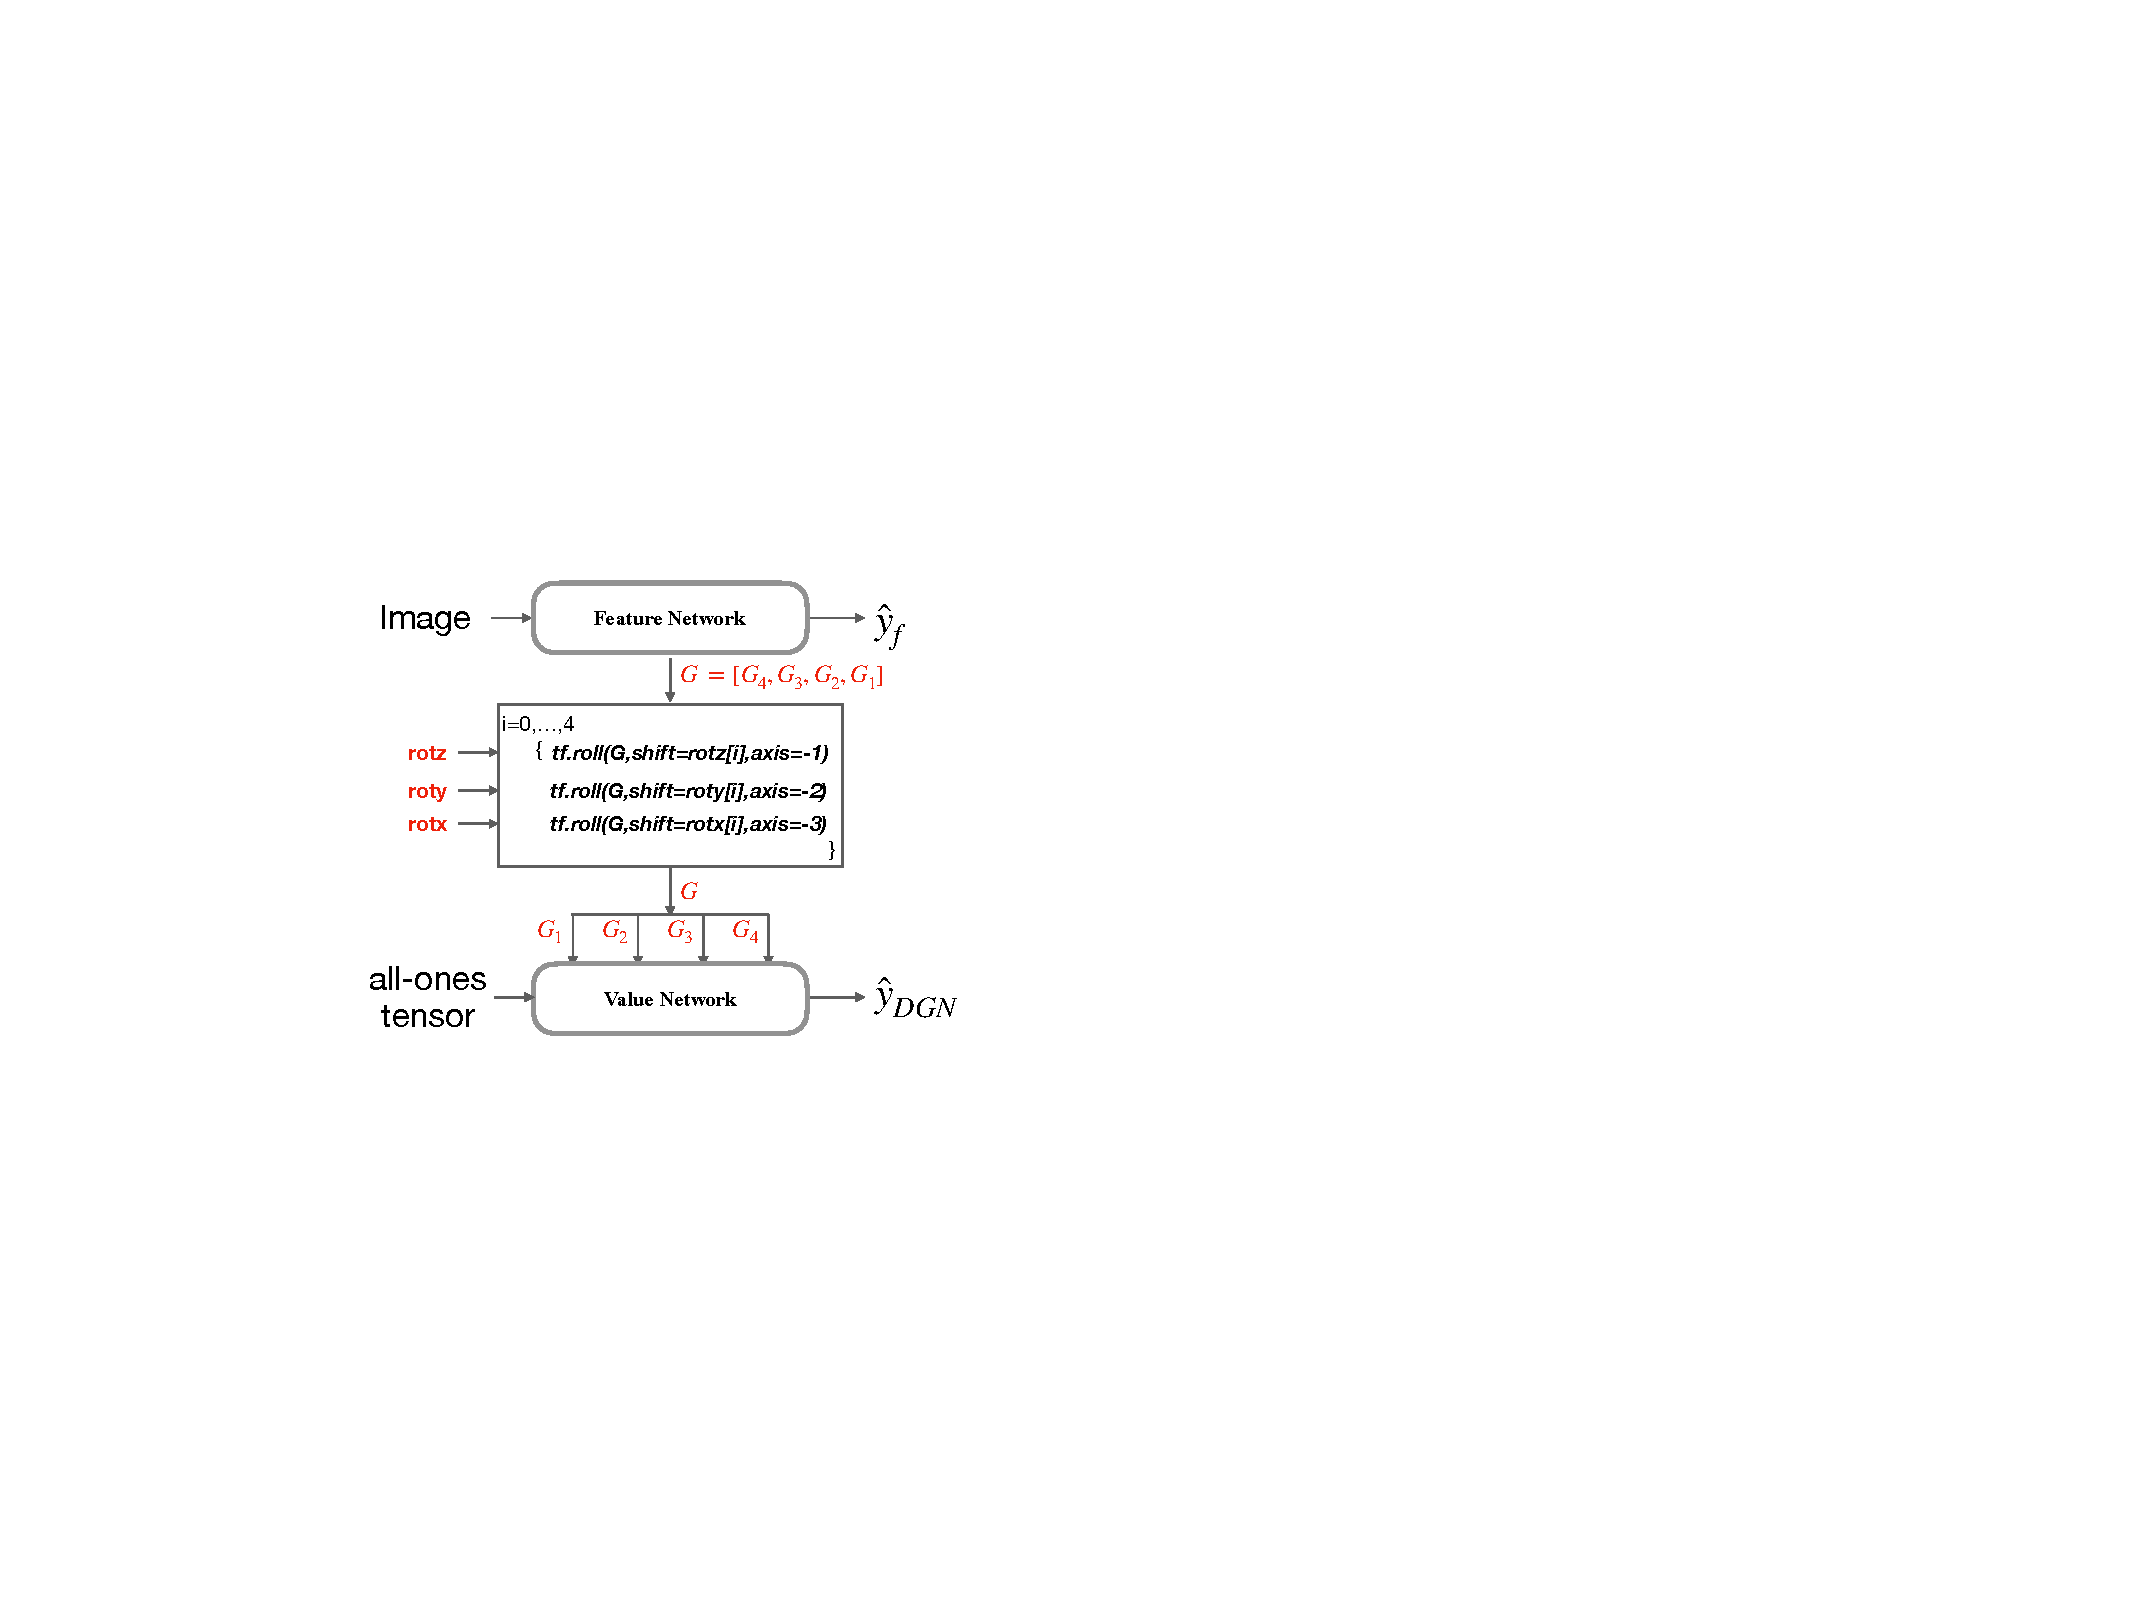
\includegraphics[scale=0.25]{figs/arbitrary_shift.pdf}
}
\end{minipage}
\begin{minipage}{0.68\columnwidth}
\resizebox{\columnwidth}{!}{
\begin{tabular}{c|c|cccccccc|c@{}}
&\resizebox{100pt}{!} {\Huge{Input}}& \resizebox{200pt}{!}{\Huge{Layer 1, Filter 1}}& \resizebox{200pt}{!}{\Huge{Layer 1, Filter 2}}&\resizebox{200pt}{!}{ \Huge{Layer 2, Filter 1}}& \resizebox{200pt}{!}{\Huge{Layer 2, Filter 2}}& \resizebox{200pt}{!}{\Huge{Layer 3, Filter 1}}& \resizebox{200pt}{!}{\Huge{Layer 3, Filter 2}}&\resizebox{200pt}{!}{\Huge{Layer 4, Filter 1}}& \resizebox{200pt}{!}{\Huge{Layer 4, Filter 2}}&\resizebox{180pt}{!}{\Huge{Test Acc.}}\\
\toprule
\resizebox{200pt}{!} {\shortstack{\Huge{Feature}\\\Huge Network\\\mbox{}\\\mbox{}\\\mbox{}\\\mbox{}\\\mbox{}\\\mbox{}\\\mbox{}}}&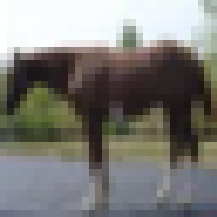
\includegraphics{visual-iclr/images/horse.png}&
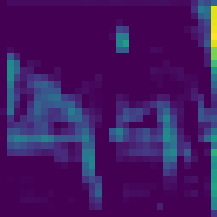
\includegraphics{images_neurips_2021/feature_network/layer_1_0.png}&
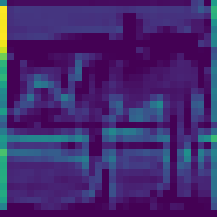
\includegraphics{images_neurips_2021/feature_network/layer_1_1.png}&
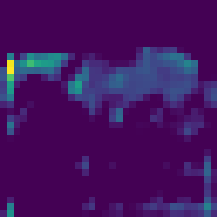
\includegraphics{images_neurips_2021/feature_network/layer_2_0.png}&
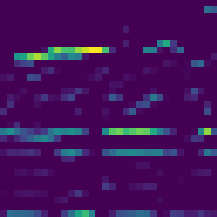
\includegraphics{images_neurips_2021/feature_network/layer_2_1.png}&
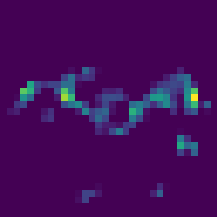
\includegraphics{images_neurips_2021/feature_network/layer_3_0.png}&
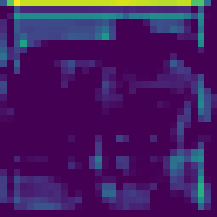
\includegraphics{images_neurips_2021/feature_network/layer_3_1.png}&
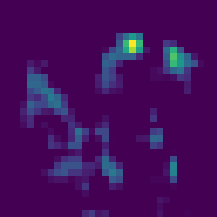
\includegraphics{images_neurips_2021/feature_network/layer_4_0.png}&
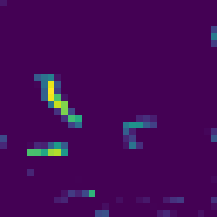
\includegraphics{images_neurips_2021/feature_network/layer_4_1.png}&
{\resizebox{200pt}{!}{\shortstack{80.4\tiny$\pm$0.3\\\mbox{}\\\mbox{}\\\mbox{}\\\mbox{}}} }\\\hline
\resizebox{200pt}{!} {\shortstack{\Huge{Value}\\\Huge Network\\\mbox{}\\\mbox{}\\\mbox{}\\\mbox{}\\\mbox{}\\\mbox{}\\\mbox{}}}&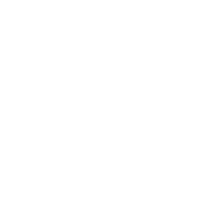
\includegraphics{images_neurips_2021/allones.png}&
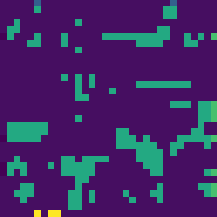
\includegraphics{images_neurips_2021/value_network//layer_1_0.png}&
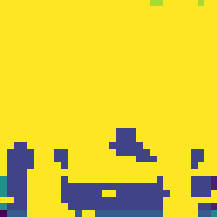
\includegraphics{images_neurips_2021/value_network//layer_1_1.png}&
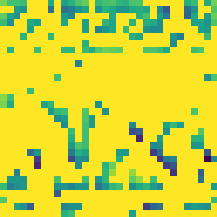
\includegraphics{images_neurips_2021/value_network//layer_2_0.png}&
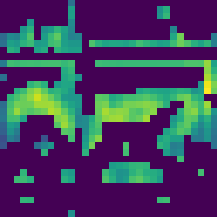
\includegraphics{images_neurips_2021/value_network//layer_2_1.png}&
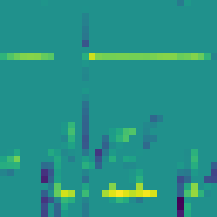
\includegraphics{images_neurips_2021/value_network//layer_3_0.png}&
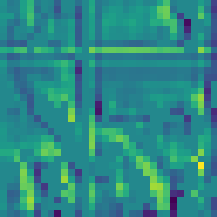
\includegraphics{images_neurips_2021/value_network//layer_3_1.png}&
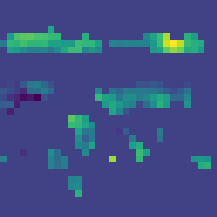
\includegraphics{images_neurips_2021/value_network//layer_4_0.png}&
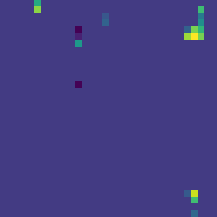
\includegraphics{images_neurips_2021/value_network//layer_4_1.png}&
{\resizebox{200pt}{!}{\shortstack{79.4 \tiny$\pm$0.2\\\mbox{}\\\mbox{}\\\mbox{}\\\mbox{}}} }\\
\end{tabular}
}

\end{minipage}
\caption{\small On the left is the setup for arbitrary rotation of gates. On the right, we have the images related to feature and value networks on top and bottom rows respectively. Each row has the input image followed by the output of first $2$ filters in each of the $4$ layers.  In the bottom row, the input column `appears' blank because it is the image of the $\mathbf{1}$ input to the value network.  Despite the arbitrary rotation and $\mathbf{1}$ input,  the value network is within $1\%$ of  feature network's test accuracy (on CIFAR-10).}
\label{fig:visual-permute}
\end{figure}

\textbf{Primal vs Dual View of features.} The standard (primal) view is that the input is processed layer-by-layer and the hidden features are in the layer outputs. 
%The dual view is that the features are encoded in the gates (analytically speaking the NPF/NPK). While both are mathematically equivalent, we believe that the dual view paints more accurate picture. 
Our experiments challenge the primal view, because, 
we do not provide the image as input but only $\mathbf{1}$ (`all-ones') as input to the value network, and we have destroyed the layer-by-layer structure of the gates before applying them as masks in the value network as well (also, the `fixed learnt' gates do not change during training). As a result, there is a huge `visual' difference between the hidden layer outputs of the feature network and that of the value network (see right of \Cref{fig:visual-permute}).  One could still insist that DNNs are so powerful that they are recovering the features layer-by-layer. Or alternatively, one can appeal to the dual view to conclude that since neither `all-ones' input nor the arbitrary rotation of the gates affect the correlation of gates (\Cref{th:main}), the performance does not degrade. While the gates are generated layer-by-layer in the feature network, when applied as masks, the function of the gates is to select and train the sub-networks corresponding to each example (viewpoint trivially following from \Cref{prop:npf-npv}) .
\begin{comment}
\textbf{Primal vs Dual View of features.} The standard (primal) view is that the input is processed layer-by-layer and the hidden features are in the layer outputs. To challenge this view, 
%The dual view is that the features are encoded in the gates (analytically speaking the NPF/NPK). While both are mathematically equivalent, we believe that the dual view paints more accurate picture. Our experiments challenge the primal view. 
we do not provide the image as input but only $\mathbf{1}$ (`all-ones') as input to the value network. Now, it could be argued that the value network gets the information about the via its gating masks. To counter this argument, we have destroyed the layer-by-layer structure of the gates before applying them as masks in the value network as well. As a result, there is a huge `visual' difference between the hidden layer outputs of the feature network and that of the value network (see right of \Cref{fig:visual-permute}).  One could still insist that DNNs are so powerful that they are recovering the features layer-by-layer. Or alternatively, one can appeal to the dual view to conclude that since neither `all-ones' input nor the arbitrary rotation of the gates affect the correlation of gates (\Cref{th:main}), the performance does not degrade. While the gates are generated layer-by-layer in the feature network, when applied as masks, the function of the gates is to learn and train the paths and sub-networks (viewpoint trivially following from \Cref{prop:npf-npv}) .
\end{comment}

\textbf{Gate learning need not be layer-by-layer.} In `decoupled learning' (\Cref{tb:regimes}), while the gates are generated layer-by-layer in the feature network, after arbitrary rotations they end in a different location in the value network during training, i.e., the gates can be arbitrarily placed while learning.

\subsection{DGN No ACT on CIFAR-10 and CIFAR-100}\label{sec:dgn-no-act-cifar}

